%\documentclass[a4paper, twoside, 12pt]{report}
%\documentclass[a5paper, 12pt, landscape]{article}
\documentclass[oneside]{article}
%\usepackage[paperwidth=400pt, paperheight=300pt, margin=40pt]{geometry}
\usepackage[paperwidth=400pt, paperheight=300pt, textwidth=360pt, textheight=280pt, top=15pt]{geometry}
%\usepackage[pdftex]{graphicx}
\usepackage{graphicx}
\graphicspath{{../obr/}{../obr/plots}}
\DeclareGraphicsExtensions{.ps, .eps}
\usepackage[slovak]{babel}
\usepackage[utf8]{inputenc} 
%\usepackage[T1]{fontenc}

\usepackage{amsmath}

\usepackage{listings}
\lstset{basicstyle=\ttfamily\footnotesize, breaklines=true}

%\usepackage[hidelinks]{hyperref}
\usepackage[breaklinks]{hyperref}

\usepackage{color} % kvoli epslatex obrazkom z octave

\usepackage{lettrine}

\usepackage{microtype}
%\usepackage[activate={true,nocompatibility},final,tracking=true,kerning=true,spacing=true,factor=1100,stretch=10,shrink=10]{microtype}
% activate={true,nocompatibility} - activate protrusion and expansion
% final - enable microtype; use ``draft'' to disable
% tracking=true, kerning=true, spacing=true - activate these techniques
% factor=1100 - add 10% to the protrusion amount (default is 1000)
% stretch=10, shrink=10 - reduce stretchability/shrinkability (default is 20/20)

%\usepackage[section]{placeins}
%\usepackage{placeins}

%\usepackage{boisik}
%\usepackage{baskervald}
\usepackage{fourier}
%\usepackage{baskervald}
%\usepackage[charter]{mathdesign}
\usepackage{Baskervaldx}	% funguje aj smallcaps: \textsc 
%\usepackage[lining]{ebgaramond}	% lining - cisla nie oldstyle
%\usepackage{concmath}
%\usepackage[charter]{mathdesign}

%\usepackage[lf]{Baskervaldx} % lining figures
%\usepackage[bigdelims,vvarbb]{newtxmath} % math italic letters from Nimbus Roman
%\usepackage[cal=boondoxo]{mathalfa} % mathcal from STIX, unslanted a bit
%\renewcommand*\oldstylenums[1]{\textosf{#1}}

%\usepackage[urw-garamond]{mathdesign}
%\usepackage[T1]{fontenc}

%\pagestyle{headings}

%% velkost fontu pod obrazkom mensia, vratane ``Obr. X:''
%\renewcommand{\figurename}{sjls} % toto nefunguje pri pouzivani babel
\addto\captionsslovak{\renewcommand{\figurename}{\small Obr.}}
%\renewcommand{\thefigure}{\small \arabic{figure}}
%\renewcommand{\thefigure}{\small \arabic{chapter}.\arabic{figure}}
\renewcommand{\thefigure}{\small \thechapter.\arabic{figure}}


\newcommand{\dif}{\, \mathrm{d}}	% diferencia (na derivacie)
\newcommand{\difp}{\partial}		% parc. diferencia 
\newcommand{\dxdt}[2]{\frac{\mathrm{d} #1}{\mathrm{d} #2}}
\newcommand{\dxdtp}[2]{\frac{\partial #1}{\partial #2}}
\newcommand{\un}[1]{\, \mathrm{#1}}	% jednotky velicin, v math mode
\newcommand{\E}[1]{\cdot 10^{#1}}
\newcommand{\degree}{^\circ}
\newcommand{\diameter}{\emptyset}
\newcommand{\cpx}{\widehat}		% komplexne fazory
\newcommand{\Ohm}{\Omega}


\newcounter{myasscount}
\renewcommand{\themyasscount}{\alph{myasscount}}
%\setcounter{myasscount}{1}
\newenvironment{myass}
{

	\refstepcounter{myasscount}
	\par
	\vspace{6pt}
	%\indent	% netreba, ked predchadza \par
	\begin{tabular}{p{.22\textwidth}  p{.68\textwidth} }
	\textbf{Predpoklad (\themyasscount)}	&
}
{
	\end{tabular}
	\par 
	\vspace{6pt}
}

\newcommand{\myfig}[3]
{
    \begin{figure}[!ht]
	\centering
	\includegraphics{#1}
	\caption{#2}
	%\label{fig:#3}
	#3
    \end{figure}
}

\newcommand{\myfigtex}[3]
{
    \begin{figure}[!ht]
	\centering
	\input{#1}
	\caption{#2}
	%\label{fig:#3}
	#3
    \end{figure}
}


\newcommand{\xcll}[2]{\def#1{\ifmmode \text{#2} \else #2 \fi}}

\xcll{\llgt}{$t$}
\xcll{\llgUd}{$U_d$}
\xcll{\llgton}{$t_{on}$}
\xcll{\llgtoff}{$t_{off}$}

\xcll{\llgTonj}{$T_{on,1}$}
\xcll{\llgToffj}{$T_{off,1}$}
\xcll{\llgTond}{$T_{on,2}$}
\xcll{\llgtj}{$t_1$}
\xcll{\llgtd}{$t_2$}

\xcll{\llgvg}{$u_G$}
\xcll{\llgvce}{$u_{CE}$}
\xcll{\llgvL}{$u_L$}
\xcll{\llgic}{$i_C$}
\xcll{\llgiD}{$i_D$}
\xcll{\llgiL}{$i_L$}
\xcll{\llgiK}{$i_K$}
\xcll{\llgIc}{$I_C$}

\xcll{\llUmerBmax}{$\approx B_{max}$}

%% prudove_trafo_model
\xcll{\llgud}{$u_2$}
\xcll{\llgij}{$i_1$}
\xcll{\llgudb}{$u_2^,$}
\xcll{\llgidk}{$i_{2,K}$}
\xcll{\llgimag}{$i_\mu$}

\xcll{\llgRcu}{$R_{Cu}$}
\xcll{\llgRb}{$R_b$}

% % % % % % % % % % 
%%% model %%%
\xcll{\llgxi}{$x_i$}
\xcll{\llgxio}{$x_{i+1}$}
\xcll{\llgyj}{$y_j$}
\xcll{\llgyjo}{$y_{j+1}$}
\xcll{\llgfij}{$f_{i,j}$}
\xcll{\llgfioj}{$f_{i+1,j}$}
\xcll{\llgfijo}{$f_{i,j+1}$}
\xcll{\llgfiojo}{$f_{i+1,j+1}$}




\xcll{\llaR}{R$\cdot \dif x$}
\xcll{\llaL}{L$\cdot \dif x$}
\xcll{\llaG}{G$\cdot \dif x$}
\xcll{\llaC}{C$\cdot \dif x$}
\xcll{\llai}{$i$}
\xcll{\llau}{$u$}
\xcll{\llaidi}{$i + \dxdtp{i}{x} \dif x$}
\xcll{\llaudu}{$u + \dxdtp{u}{x} \dif x$}
\xcll{\llaGen}{generátor}
\xcll{\llaZat}{spotrebič}
\xcll{\lladx}{$\dif x$}




%%%%%%%%%%%%%%%%%%%%%%%%%%%%%%%%%%%%%%%%%%%%%%%%%%%%%%%%%%%%%%%%%%%%%%%%%%%%%%%%%%%%%
%%%%%%%%%%%%%%%%%%%%%%%%%%%%%%%%%%%%%%%%%%%%%%%%%%%%%%%%%%%%%%%%%%%%%%%%%%%%%%%%%%%%%

\begin{document}

\author{Ján Mikláš,\\vedúci práce: doc. Dr. Ing. Miroslav Patočka}
\date{Jún 2016}
\title{\vspace{60pt}Výkonové spínacie tranzistory}
\maketitle

%\setcounter{page}{7}

\newpage
\tableofcontents

\newpage
\section{Vytýčené ciele}
\begin{itemize}
    \item Dôveryhodné meranie spínacích priebehov na tranzistorovom spínači
    \item Model $g_{CE}(t)$ - zostavenie, overenie, simulácie
\end{itemize}

{\centering 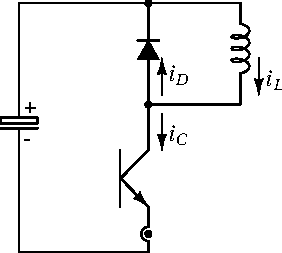
\includegraphics[scale=.8]{obr/tranzistorovy_spinac} \par}

\newpage
{\centering \section{Meranie} \label{sec:meranie} \par}

%\newpage
\subsection{Metóda - double-shot}
{\centering
	\begin{tabular}{p{.4\textwidth}  p{.6\textwidth} }
	\vspace{-5.5cm} 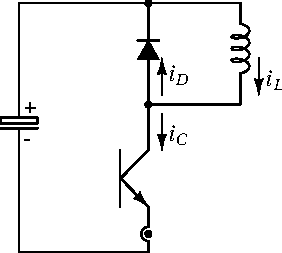
\includegraphics[scale=.8]{obr/tranzistorovy_spinac}
	&
    	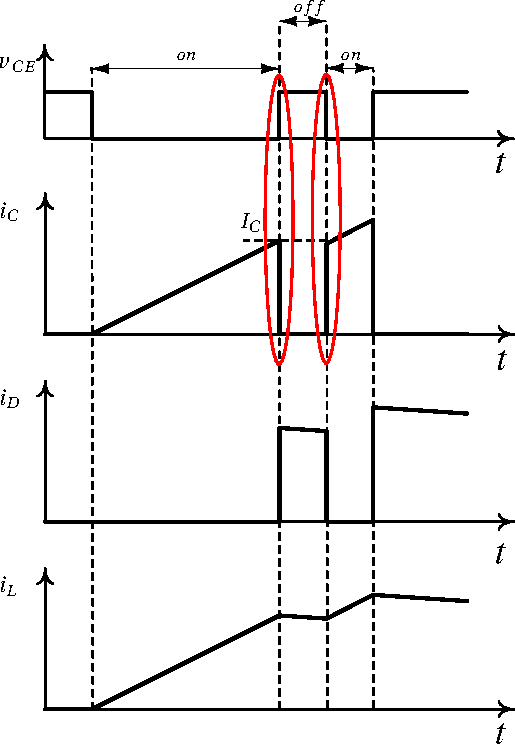
\includegraphics[scale=.6]{obr/priebehy_doubleshot} \newline
    \end{tabular}
}

\subsection{Meracie pracovisko}

{\centering 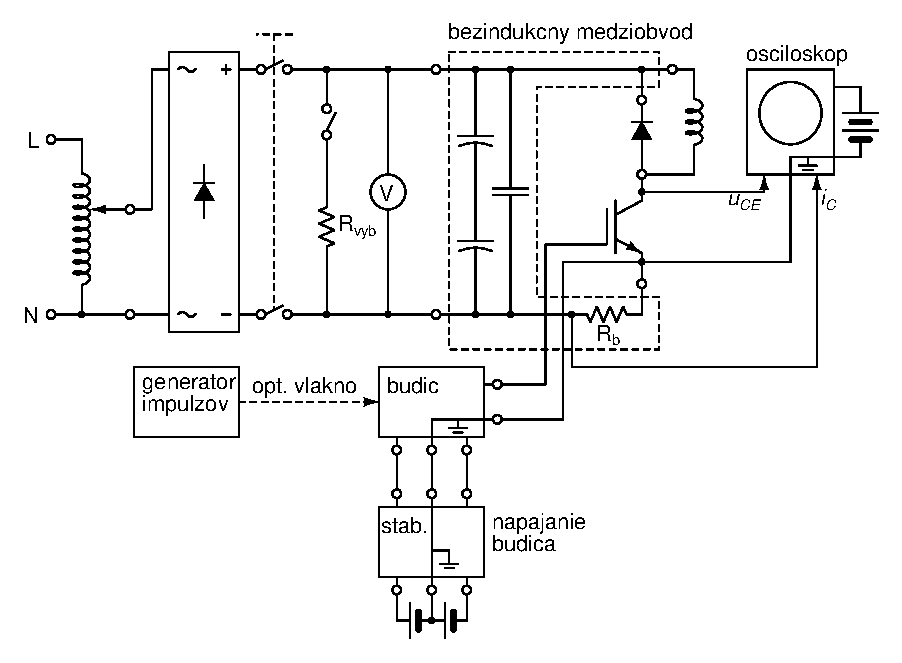
\includegraphics[height=.9\textheight]{schema_pracovisko} \par }


%%%%%%%%%%%%%%%%%%%%%%%%%%%%%%%%%%%%%%%%%%%%%%%%%%%%%%%%%%%%%%%%%%%%%%%%%%%%%%%%%


{\centering \section{Model $g_{CE}(t)$} \label{sec:model} }

{\centering % XCircuit output "BJT_iv_indukc.tex" for LaTeX input from BJT_iv_indukc.ps
\def\putbox#1#2#3#4{\makebox[0in][l]{\makebox[#1][l]{}\raisebox{\baselineskip}[0in][0in]{\raisebox{#2}[0in][0in]{\scalebox{#3}{#4}}}}}
\def\rightbox#1{\makebox[0in][r]{#1}}
\def\centbox#1{\makebox[0in]{#1}}
\def\topbox#1{\raisebox{-0.60\baselineskip}[0in][0in]{#1}}
\def\midbox#1{\raisebox{-0.20\baselineskip}[0in][0in]{#1}}
   \scalebox{0.8}{
   \normalsize
   \parbox{4.36979in}{
   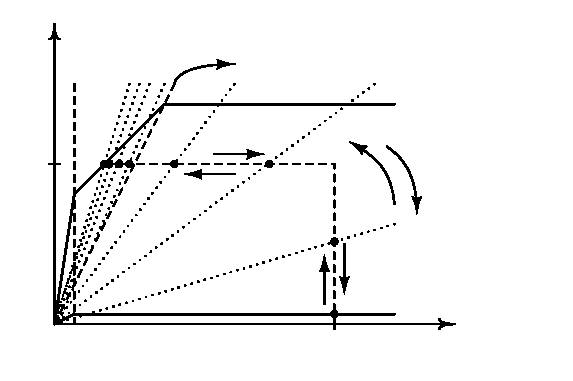
\includegraphics[scale=1.25]{BJT_iv_indukc}\\
   % translate x=287 y=291 scale 0.30
   \putbox{0.06in}{2.50in}{1.20}{$I_C$}%
   \putbox{3.40in}{0.09in}{1.20}{$U_{CE}$}%
   \putbox{1.90in}{2.50in}{1.20}{odpor drift. oblasti}%
   \putbox{3.23in}{2.17in}{1.20}{$I_{B,on}$}%
   \putbox{3.34in}{1.61in}{1.20}{$g_{CE}(t)$}%
   \putbox{1.73in}{1.84in}{1.20}{vyp.}%
   \putbox{1.31in}{1.42in}{1.20}{zap.}%
   \putbox{0.06in}{1.63in}{1.20}{$I_L$}%
   \putbox{2.56in}{0.13in}{1.20}{$U_d$}%
   } % close 'parbox'
   } % close 'scalebox'
   \vspace{-\baselineskip} % this is not necessary, but looks better
 \par}

\begin{itemize}
    \item predpokl. priebeh nezávislý na kolektorovom obvode (trajektórii prac. bodu)
    \item nezávislý na $U_d$
    \item závislý na $I_L$, $i_B(t)$, \ldots
\end{itemize}


\subsection{Aproximácia $g_{CE}(t)$ analytickou funkciou}
\begin{equation}
	\begin{array}{c | c c c}
		t & t_0 & t_1 & t_2 \\
		\hline
		g(t) & G_0 & G_1 & G_2
	\end{array}
	\label{eq:tab_predpis_t012}
\end{equation}

\begin{figure}[ht!]
	\centering
	% XCircuit output "krivka_vyp_t012.tex" for LaTeX input from krivka_vyp_t012.ps
\def\putbox#1#2#3#4{\makebox[0in][l]{\makebox[#1][l]{}\raisebox{\baselineskip}[0in][0in]{\raisebox{#2}[0in][0in]{\scalebox{#3}{#4}}}}}
\def\rightbox#1{\makebox[0in][r]{#1}}
\def\centbox#1{\makebox[0in]{#1}}
\def\topbox#1{\raisebox{-0.60\baselineskip}[0in][0in]{#1}}
\def\midbox#1{\raisebox{-0.20\baselineskip}[0in][0in]{#1}}
   \scalebox{0.8}{
   \normalsize
   \parbox{2.35417in}{
   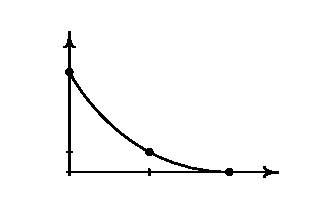
\includegraphics[scale=1.25]{krivka_vyp_t012}\\
   % translate x=-9 y=147 scale 0.30
   \putbox{0.06in}{1.34in}{1.20}{$g(t)$}%
   \putbox{2.11in}{0.09in}{1.20}{$t$}%
   \putbox{1.69in}{0.09in}{1.20}{$t_2$}%
   \putbox{1.02in}{0.09in}{1.20}{$t_1$}%
   \putbox{0.36in}{0.09in}{1.20}{$t_0$}%
   \putbox{0.15in}{0.21in}{1.20}{$G_2$}%
   \putbox{0.15in}{0.38in}{1.20}{$G_1$}%
   \putbox{0.15in}{1.04in}{1.20}{$G_0$}%
   } % close 'parbox'
   } % close 'scalebox'
   \vspace{-\baselineskip} % this is not necessary, but looks better

	\caption{príklad krivky pre vypínací dej}
	\label{fig:krivka_vyp_t012}
\end{figure}

\begin{equation}
	g_{CE}(t) = 
	\left\{
	\begin{array}{l l}
		G_0;	& t<t_0 \\
		g_1(t);	& t_0 \leq t < t_1 \\
		g_2(t);	& t_1 \leq t < t_2 \\
		G_2;		& t \geq t_2
	\end{array}
	\right.
\end{equation}

\begin{itemize}
    \item funkcie $g_i(t)$ definované vhodnou aproximáciou a okrajovými podmienkami ($g_i(t_{i-1}) = G_{i-1}$; $g_i(t_i) = G_i$; hladkosť: $g'_i(t_i) = g'_{i+1}(t_i)$)
\end{itemize}


\subsection{Vplyv parazitných prvkov - indukčnosť} \label{subsec:parazity}
{ \centering
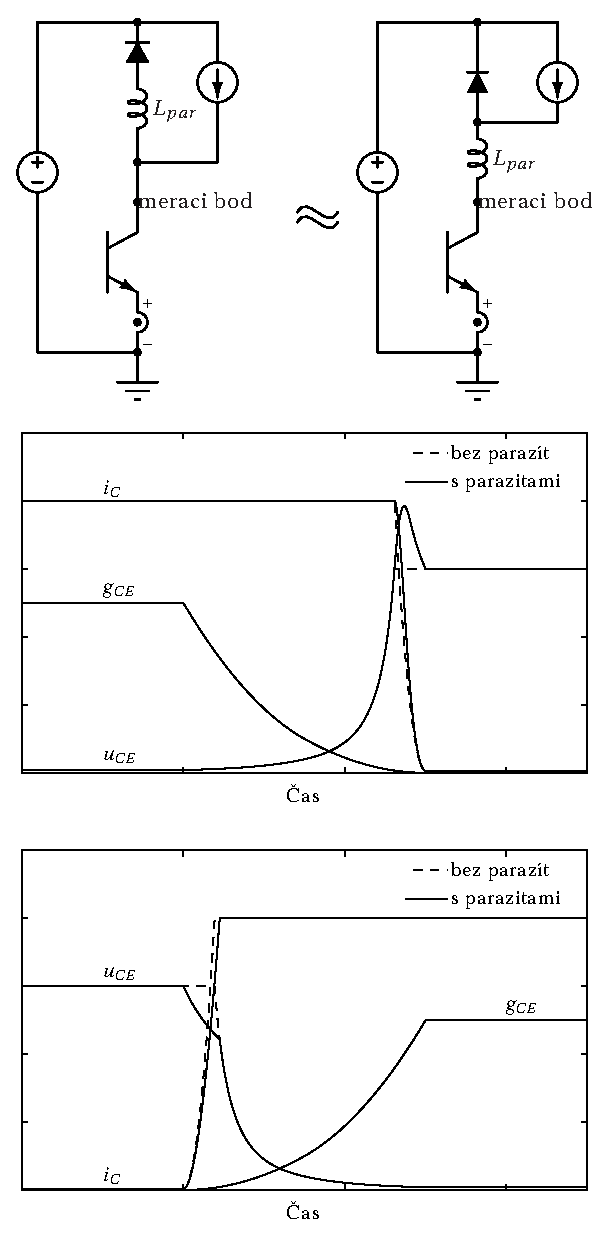
\includegraphics[height=.85\textheight]{obr/Lpar_prekmit}
\hspace{36pt}
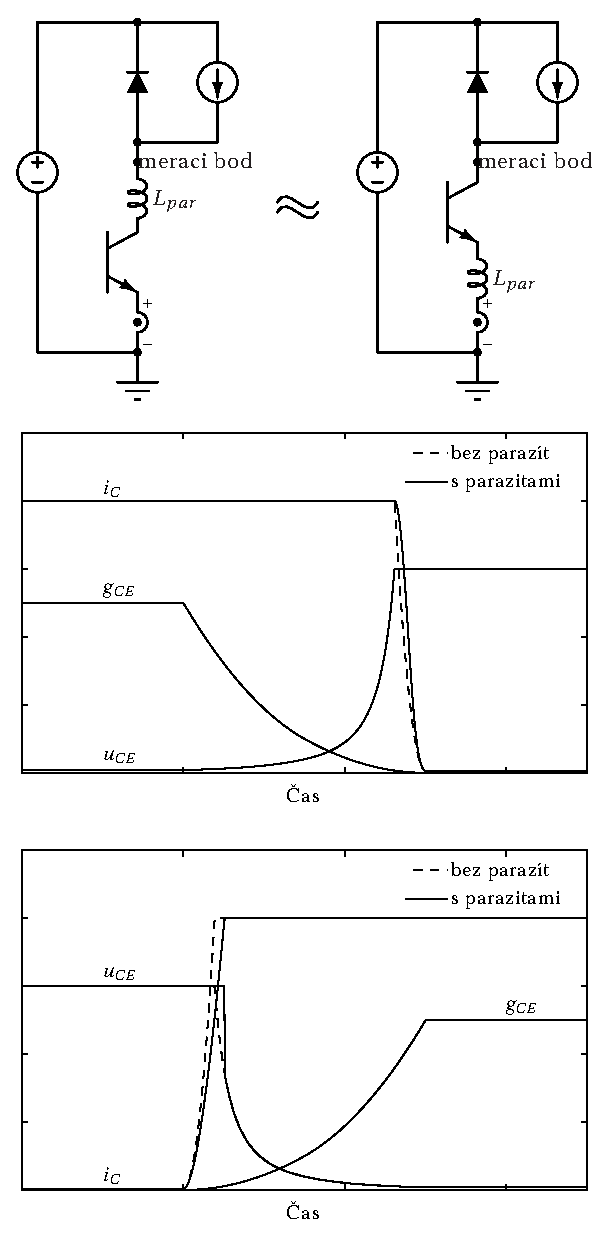
\includegraphics[height=.85\textheight]{obr/Lpar_bez_prekmitu}
\par }

\subsection{Vplyv parazitných prvkov - kapacita} \label{subsec:parazity}
{ \centering
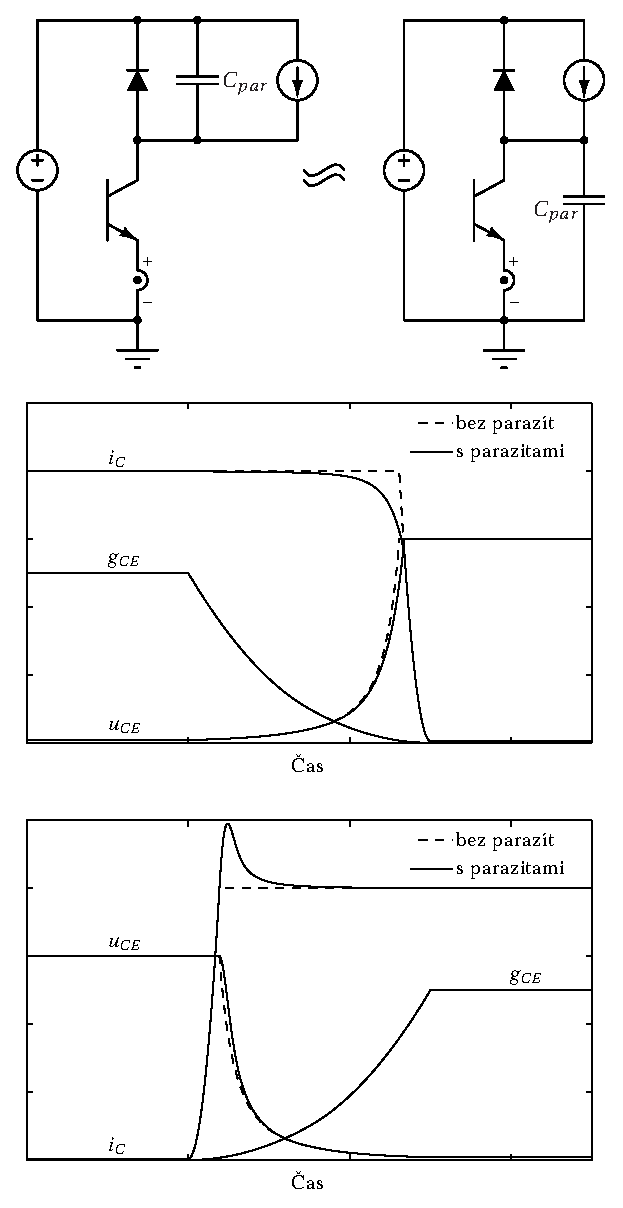
\includegraphics[height=.85\textheight]{obr/Cpar_prekmit}
\hspace{36pt}
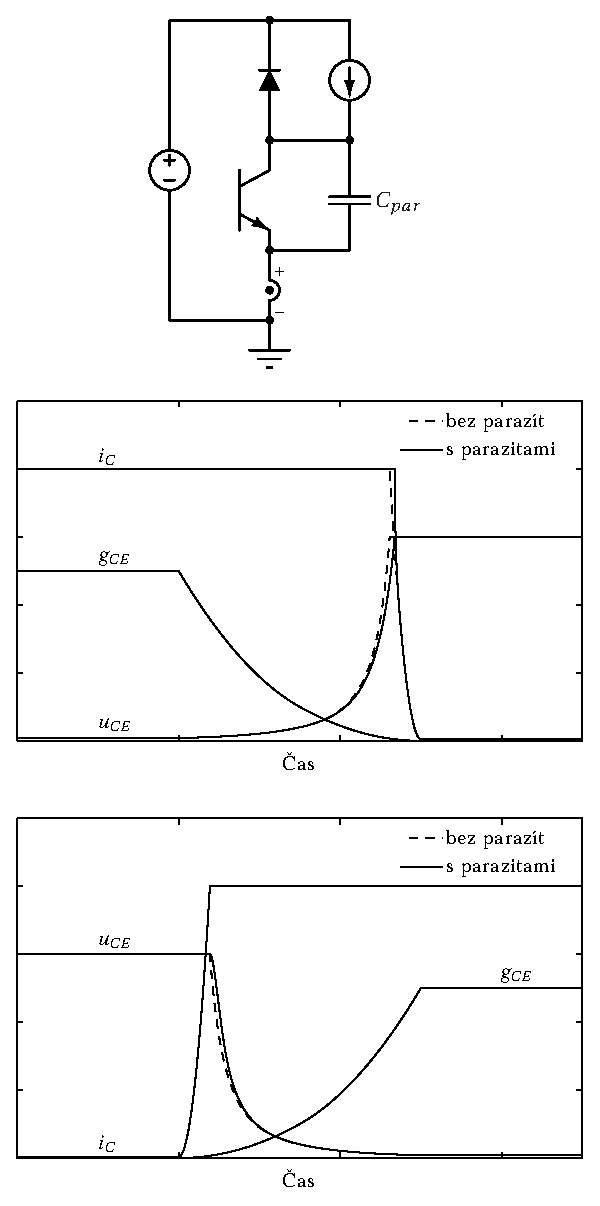
\includegraphics[height=.85\textheight]{obr/Cpar_bez_prekmitu}
\par }


%%%%%%%%%%%%%%%%%%%%%%%%%%%%%%%%%%%%%%%%%%%%%%%%%%%%%%%%%%%%%%%%%%%%%%%%%%%%%%%%%%


\newpage
{\centering \section{Výsledky meraní a simulácii} }


\centering

\subsubsection*{Nezávislosť $t_{off}$ ($g_{CE}$) na napätí $U_d$}
% Title: glps_renderer figure
% Creator: GL2PS 1.3.8, (C) 1999-2012 C. Geuzaine
% For: Octave
% CreationDate: Thu May 26 13:49:05 2016
\setlength{\unitlength}{1pt}
\begin{picture}(0,0)
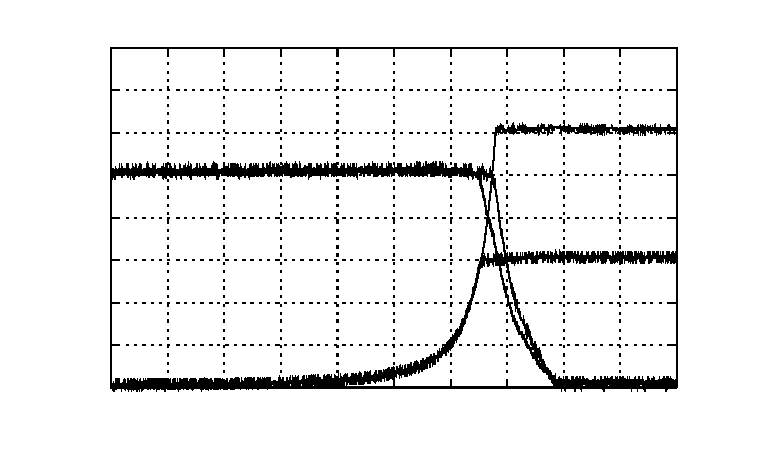
\includegraphics{../../latex/obr/plots/bjt_porov_300V_150V_off-inc}
\end{picture}%
\begin{picture}(350,200)(0,0)
\fontsize{10}{0}
\selectfont\put(181.125,17){\makebox(0,0)[t]{\textcolor[rgb]{0,0,0}{{$200\un{ns/div}$}}}}
\fontsize{10}{0}
\selectfont\put(36.4954,103.5){\rotatebox{90}{\makebox(0,0)[b]{\textcolor[rgb]{0,0,0}{{$50\un{V/div},\,\,\, 2\un{A/div}$}}}}}
\fontsize{10}{0}
\selectfont\put(262.5,156.475){\makebox(0,0)[l]{\textcolor[rgb]{0,0,0}{{$u_{CE} = 300\un{V}$}}}}
\fontsize{10}{0}
\selectfont\put(262.5,95.35){\makebox(0,0)[l]{\textcolor[rgb]{0,0,0}{{$u_{CE} = 150\,\mathrm{V}$}}}}
\fontsize{10}{0}
\selectfont\put(99.75,136.1){\makebox(0,0)[l]{\textcolor[rgb]{0,0,0}{{$i_{C} = 10\un{A}$}}}}
\end{picture}


\subsubsection*{Závislosť $t_{off}$, ($g_{CE}$) na prúde $I_L$}
% Title: glps_renderer figure
% Creator: GL2PS 1.3.8, (C) 1999-2012 C. Geuzaine
% For: Octave
% CreationDate: Fri May 27 10:10:43 2016
\setlength{\unitlength}{1pt}
\begin{picture}(0,0)
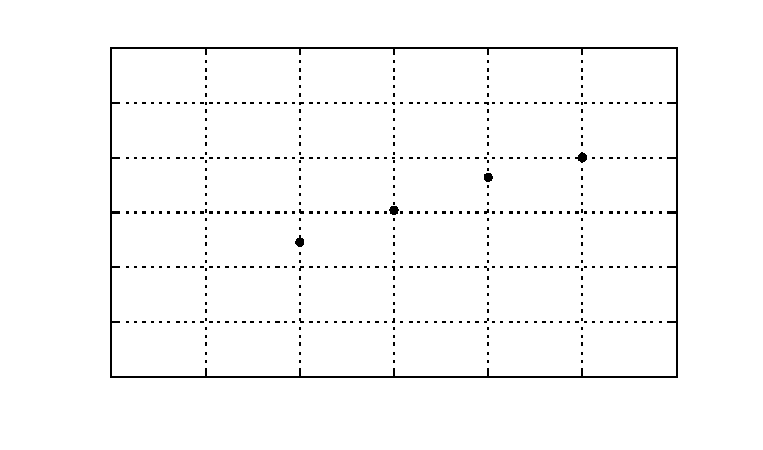
\includegraphics{../../latex/obr/plots/bjt_tfi-inc}
\end{picture}%
\begin{picture}(350,200)(0,0)
\fontsize{10}{0}
\selectfont\put(45.5,22){\makebox(0,0)[t]{\textcolor[rgb]{0,0,0}{{0}}}}
\fontsize{10}{0}
\selectfont\put(90.7083,22){\makebox(0,0)[t]{\textcolor[rgb]{0,0,0}{{2}}}}
\fontsize{10}{0}
\selectfont\put(135.917,22){\makebox(0,0)[t]{\textcolor[rgb]{0,0,0}{{4}}}}
\fontsize{10}{0}
\selectfont\put(181.125,22){\makebox(0,0)[t]{\textcolor[rgb]{0,0,0}{{6}}}}
\fontsize{10}{0}
\selectfont\put(226.333,22){\makebox(0,0)[t]{\textcolor[rgb]{0,0,0}{{8}}}}
\fontsize{10}{0}
\selectfont\put(271.542,22){\makebox(0,0)[t]{\textcolor[rgb]{0,0,0}{{10}}}}
\fontsize{10}{0}
\selectfont\put(316.75,22){\makebox(0,0)[t]{\textcolor[rgb]{0,0,0}{{12}}}}
\fontsize{10}{0}
\selectfont\put(40.4954,27){\makebox(0,0)[r]{\textcolor[rgb]{0,0,0}{{0}}}}
\fontsize{10}{0}
\selectfont\put(40.4954,53.3333){\makebox(0,0)[r]{\textcolor[rgb]{0,0,0}{{0.5}}}}
\fontsize{10}{0}
\selectfont\put(40.4954,79.6667){\makebox(0,0)[r]{\textcolor[rgb]{0,0,0}{{1}}}}
\fontsize{10}{0}
\selectfont\put(40.4954,106){\makebox(0,0)[r]{\textcolor[rgb]{0,0,0}{{1.5}}}}
\fontsize{10}{0}
\selectfont\put(40.4954,132.333){\makebox(0,0)[r]{\textcolor[rgb]{0,0,0}{{2}}}}
\fontsize{10}{0}
\selectfont\put(40.4954,158.667){\makebox(0,0)[r]{\textcolor[rgb]{0,0,0}{{2.5}}}}
\fontsize{10}{0}
\selectfont\put(40.4954,185){\makebox(0,0)[r]{\textcolor[rgb]{0,0,0}{{3}}}}
\fontsize{10}{0}
\selectfont\put(181.125,11){\makebox(0,0)[t]{\textcolor[rgb]{0,0,0}{{$I_C (\un{A})$}}}}
\fontsize{10}{0}
\selectfont\put(21.4954,106){\rotatebox{90}{\makebox(0,0)[b]{\textcolor[rgb]{0,0,0}{{$t_{off} (\un{\mu s})$}}}}}
\end{picture}


\subsubsection*{Vypínací dej - BJT, $300\un{V}$, $10\un{A}$}
% Title: glps_renderer figure
% Creator: GL2PS 1.3.8, (C) 1999-2012 C. Geuzaine
% For: Octave
% CreationDate: Thu May 26 12:39:38 2016
\setlength{\unitlength}{1pt}
\begin{picture}(0,0)
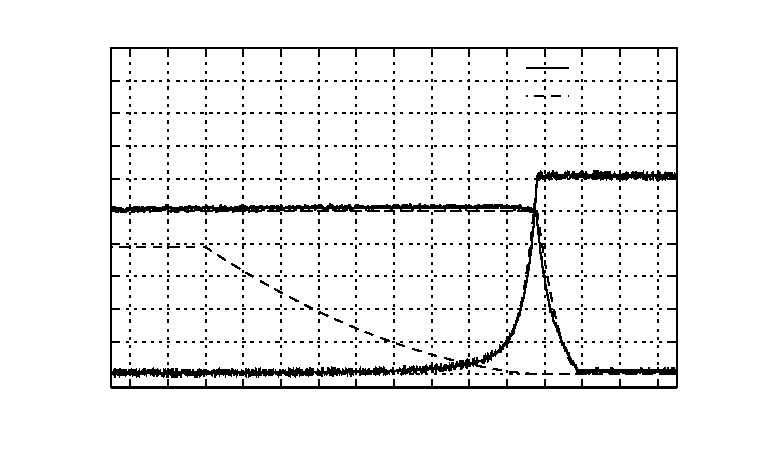
\includegraphics{plots/bjt_300_10_off-inc}
\end{picture}%
\begin{picture}(350,200)(0,0)
\fontsize{10}{0}
\selectfont\put(181.126,17){\makebox(0,0)[t]{\textcolor[rgb]{0,0,0}{{(200ns / div)}}}}
\fontsize{10}{0}
\selectfont\put(36.4957,103.5){\rotatebox{90}{\makebox(0,0)[b]{\textcolor[rgb]{0,0,0}{{(50V / div),
(2A / div),
(2S / div)}}}}}
\fontsize{10}{0}
\selectfont\put(54.5426,95.665){\makebox(0,0)[l]{\textcolor[rgb]{0,0,0}{{$g_{CE}$}}}}
\fontsize{10}{0}
\selectfont\put(54.5426,34.9528){\makebox(0,0)[l]{\textcolor[rgb]{0,0,0}{{$u_{CE}$}}}}
\fontsize{10}{0}
\selectfont\put(54.5426,114.706){\makebox(0,0)[l]{\textcolor[rgb]{0,0,0}{{$i_{C}$}}}}
\fontsize{10}{0}
\selectfont\put(267.403,175.49){\makebox(0,0)[l]{\textcolor[rgb]{0,0,0}{{meranie}}}}
\fontsize{10}{0}
\selectfont\put(267.403,161.816){\makebox(0,0)[l]{\textcolor[rgb]{0,0,0}{{simulácia}}}}
\end{picture}


\subsubsection*{Zapínací dej - BJT, $300\un{V}$, $10\un{A}$}
%% Title: glps_renderer figure
% Creator: GL2PS 1.3.8, (C) 1999-2012 C. Geuzaine
% For: Octave
% CreationDate: Tue Jun  7 21:02:38 2016
\setlength{\unitlength}{1pt}
\begin{picture}(0,0)
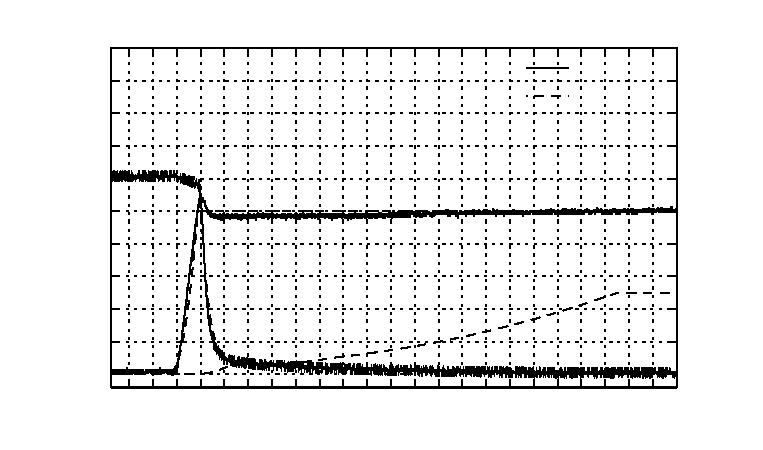
\includegraphics{../../latex/obr/plots/bjt_300_10_on-inc}
\end{picture}%
\begin{picture}(350,200)(0,0)
\fontsize{10}{0}
\selectfont\put(181.125,17){\makebox(0,0)[t]{\textcolor[rgb]{0,0,0}{{$200\un{ns/div}$}}}}
\fontsize{10}{0}
\selectfont\put(36.4957,103.5){\rotatebox{90}{\makebox(0,0)[b]{\textcolor[rgb]{0,0,0}{{$50\un{V/div},\,\,\, 2\un{A/div},\,\,\, 2\un{S/div}$}}}}}
\fontsize{10}{0}
\selectfont\put(311.039,73.7175){\makebox(0,0)[l]{\textcolor[rgb]{0,0,0}{{$g_{CE}$}}}}
\fontsize{10}{0}
\selectfont\put(51.2097,129.517){\makebox(0,0)[l]{\textcolor[rgb]{0,0,0}{{$u_{CE}$}}}}
\fontsize{10}{0}
\selectfont\put(51.2097,35.854){\makebox(0,0)[l]{\textcolor[rgb]{0,0,0}{{$i_{C}$}}}}
\fontsize{10}{0}
\selectfont\put(267.403,175.49){\makebox(0,0)[l]{\textcolor[rgb]{0,0,0}{{meranie}}}}
\fontsize{10}{0}
\selectfont\put(267.403,161.816){\makebox(0,0)[l]{\textcolor[rgb]{0,0,0}{{simulácia}}}}
\end{picture}

% Title: glps_renderer figure
% Creator: GL2PS 1.3.8, (C) 1999-2012 C. Geuzaine
% For: Octave
% CreationDate: Mon May 30 02:00:37 2016
\setlength{\unitlength}{1pt}
\begin{picture}(0,0)
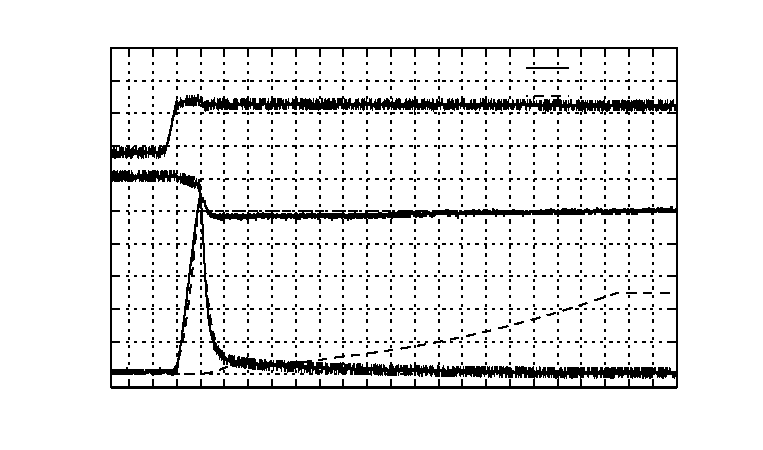
\includegraphics{../../latex/obr/plots/bjt_zap_ube-inc}
\end{picture}%
\begin{picture}(350,200)(0,0)
\fontsize{10}{0}
\selectfont\put(181.125,17){\makebox(0,0)[t]{\textcolor[rgb]{0,0,0}{{$200\un{ns/div}$}}}}
\fontsize{10}{0}
\selectfont\put(36.4957,103.5){\rotatebox{90}{\makebox(0,0)[b]{\textcolor[rgb]{0,0,0}{{$50\un{V/div},\,\,\, 2\un{A/div},\,\,\, 2\un{S/div}$}}}}}
\fontsize{10}{0}
\selectfont\put(311.039,73.7175){\makebox(0,0)[l]{\textcolor[rgb]{0,0,0}{{$g_{CE}$}}}}
\fontsize{10}{0}
\selectfont\put(51.2097,129.517){\makebox(0,0)[l]{\textcolor[rgb]{0,0,0}{{$u_{CE}$}}}}
\fontsize{10}{0}
\selectfont\put(51.2097,35.854){\makebox(0,0)[l]{\textcolor[rgb]{0,0,0}{{$i_{C}$}}}}
\fontsize{10}{0}
\selectfont\put(99.7492,163.058){\makebox(0,0)[l]{\textcolor[rgb]{0,0,0}{{$u_{BE}$}}}}
\fontsize{10}{0}
\selectfont\put(267.403,175.49){\makebox(0,0)[l]{\textcolor[rgb]{0,0,0}{{meranie}}}}
\fontsize{10}{0}
\selectfont\put(267.403,161.816){\makebox(0,0)[l]{\textcolor[rgb]{0,0,0}{{simulácia}}}}
\end{picture}

\begin{itemize}
    \item priebeh $g_{CE}(t)$ sa vymyká predstave hladkej krivky bez inflexných bodov
\end{itemize}

\newpage
\subsubsection*{BJT - Prechod z aktívnej do saturačnej oblasti}
{\centering \vspace{24pt} 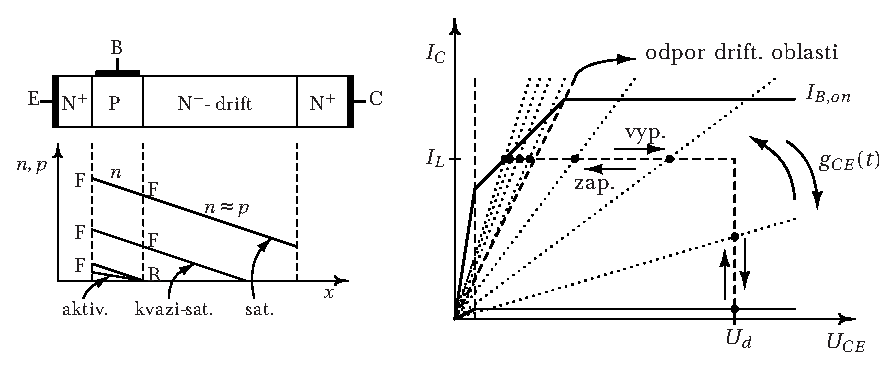
\includegraphics[width=\textwidth]{obr/oblasti} \par }

\newpage
\subsubsection*{Závislosť napätia $U_{CE,hran}$ v čase \uv{zlomu} na prúde $I_L$}
\begin{itemize}
    \item predpokladaná hranica medzi kvázi-saturačnou a aktívnou oblasťou (záverným a priepustným pólovaním prechodu báza - kolektor)
\end{itemize}
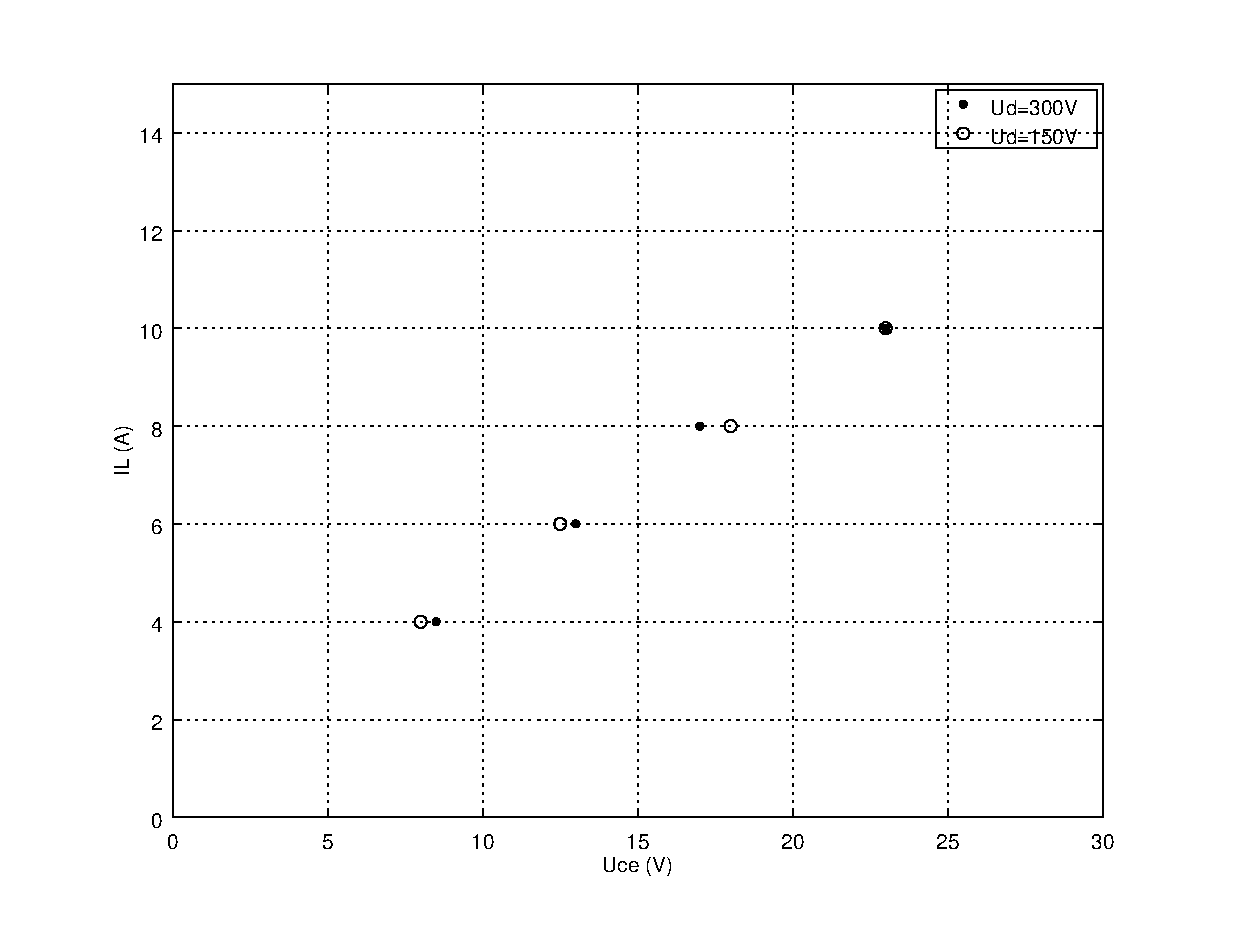
\includegraphics[height=.8\textheight]{obr/hranica_kvazisat_mozno}


\subsubsection*{Vypínací dej - IGBT, $300\un{V}$, $40\un{A}$}
% Title: glps_renderer figure
% Creator: GL2PS 1.3.8, (C) 1999-2012 C. Geuzaine
% For: Octave
% CreationDate: Mon May 30 03:13:43 2016
\setlength{\unitlength}{1pt}
\begin{picture}(0,0)
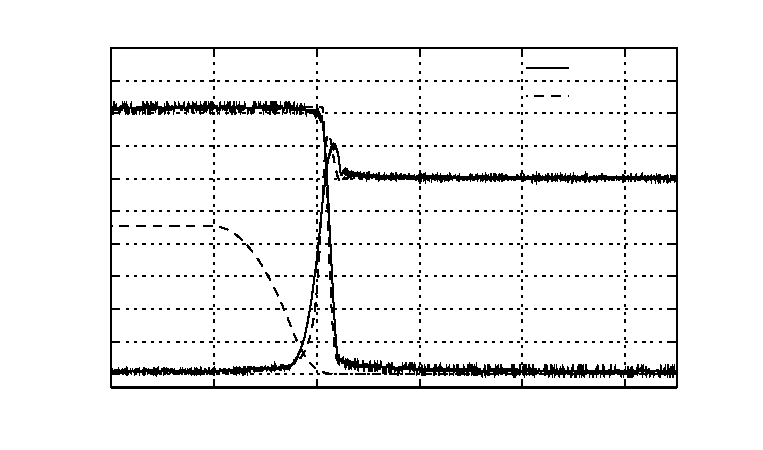
\includegraphics{../../latex/obr/plots/igbt_300_40_1_off_par-inc}
\end{picture}%
\begin{picture}(350,200)(0,0)
\fontsize{10}{0}
\selectfont\put(181.129,17){\makebox(0,0)[t]{\textcolor[rgb]{0,0,0}{{$200\un{ns/div}$}}}}
\fontsize{10}{0}
\selectfont\put(36.4978,103.5){\rotatebox{90}{\makebox(0,0)[b]{\textcolor[rgb]{0,0,0}{{$50\un{V/div},\,\,\, 5\un{A/div},\,\,\, 2\un{S/div}$}}}}}
\fontsize{10}{0}
\selectfont\put(70.1598,105.592){\makebox(0,0)[l]{\textcolor[rgb]{0,0,0}{{$g_{CE}$}}}}
\fontsize{10}{0}
\selectfont\put(70.1598,35.9559){\makebox(0,0)[l]{\textcolor[rgb]{0,0,0}{{$u_{CE}$}}}}
\fontsize{10}{0}
\selectfont\put(70.1598,156.789){\makebox(0,0)[l]{\textcolor[rgb]{0,0,0}{{$i_{C}$}}}}
\fontsize{10}{0}
\selectfont\put(267.403,175.49){\makebox(0,0)[l]{\textcolor[rgb]{0,0,0}{{meranie}}}}
\fontsize{10}{0}
\selectfont\put(267.403,161.816){\makebox(0,0)[l]{\textcolor[rgb]{0,0,0}{{simulácia}}}}
\end{picture}


\subsubsection*{Zapínací dej - IGBT, $300\un{V}$, $40\un{A}$}
% Title: glps_renderer figure
% Creator: GL2PS 1.3.8, (C) 1999-2012 C. Geuzaine
% For: Octave
% CreationDate: Mon May 30 03:13:51 2016
\setlength{\unitlength}{1pt}
\begin{picture}(0,0)
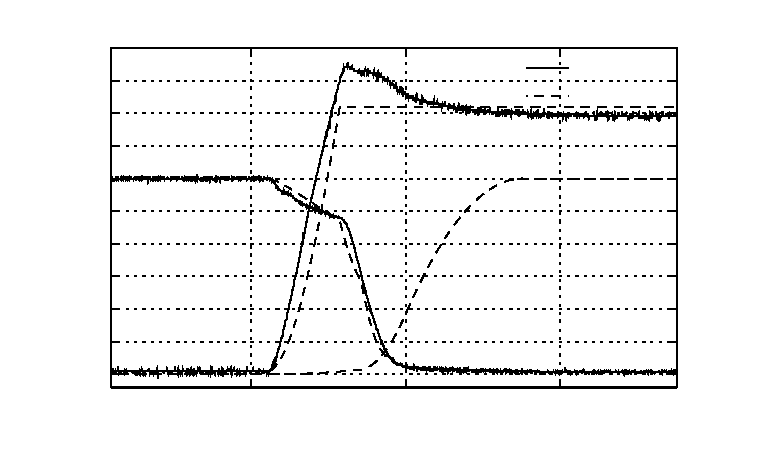
\includegraphics{../../latex/obr/plots/igbt_300_40_1_on_par-inc}
\end{picture}%
\begin{picture}(350,200)(0,0)
\fontsize{10}{0}
\selectfont\put(181.125,17){\makebox(0,0)[t]{\textcolor[rgb]{0,0,0}{{$200\un{ns/div}$}}}}
\fontsize{10}{0}
\selectfont\put(36.4937,103.5){\rotatebox{90}{\makebox(0,0)[b]{\textcolor[rgb]{0,0,0}{{$50\un{V/div},\,\,\, 5\un{A/div},\,\,\, 2\un{S/div}$}}}}}
\fontsize{10}{0}
\selectfont\put(279.591,128.58){\makebox(0,0)[l]{\textcolor[rgb]{0,0,0}{{$g_{CE}$}}}}
\fontsize{10}{0}
\selectfont\put(82.6595,129.351){\makebox(0,0)[l]{\textcolor[rgb]{0,0,0}{{$u_{CE}$}}}}
\fontsize{10}{0}
\selectfont\put(82.6595,29.9291){\makebox(0,0)[l]{\textcolor[rgb]{0,0,0}{{$i_{C}$}}}}
\fontsize{10}{0}
\selectfont\put(267.403,175.49){\makebox(0,0)[l]{\textcolor[rgb]{0,0,0}{{meranie}}}}
\fontsize{10}{0}
\selectfont\put(267.403,161.816){\makebox(0,0)[l]{\textcolor[rgb]{0,0,0}{{simulácia}}}}
\end{picture}



%%%%%%%%%%%%%%%%%%%%%%%%%%%%%%%%%%%%%%%%%%%%%%%%%%%%%%%%%%%%%%%%%%%%%%%%%%%%%%%%%%

\newpage
\section*{Záver} \label{sec:zaver} \addcontentsline{toc}{section}{Záver}
\begin{itemize}
    \item Dôveryhodnosť merania (snímané priebehy, parazitné vplyvy)
    \item Použiteľnosť modela
\end{itemize}


\section*{}
\newpage
\centering
\newpage
\vspace{60pt}
Ďakujem za pozornosť

%%%%%%%%%%%%%%%%%%%%%%%%%%%%%%%%%%%%%%%%%%%%%%%%%%%%%%%%%%%%%%%%%%%%%%%%%%%%%%%%%

\appendix

\section{Obvodová schéma budiča výkonových tranzistorov}
\hspace{-1.8cm}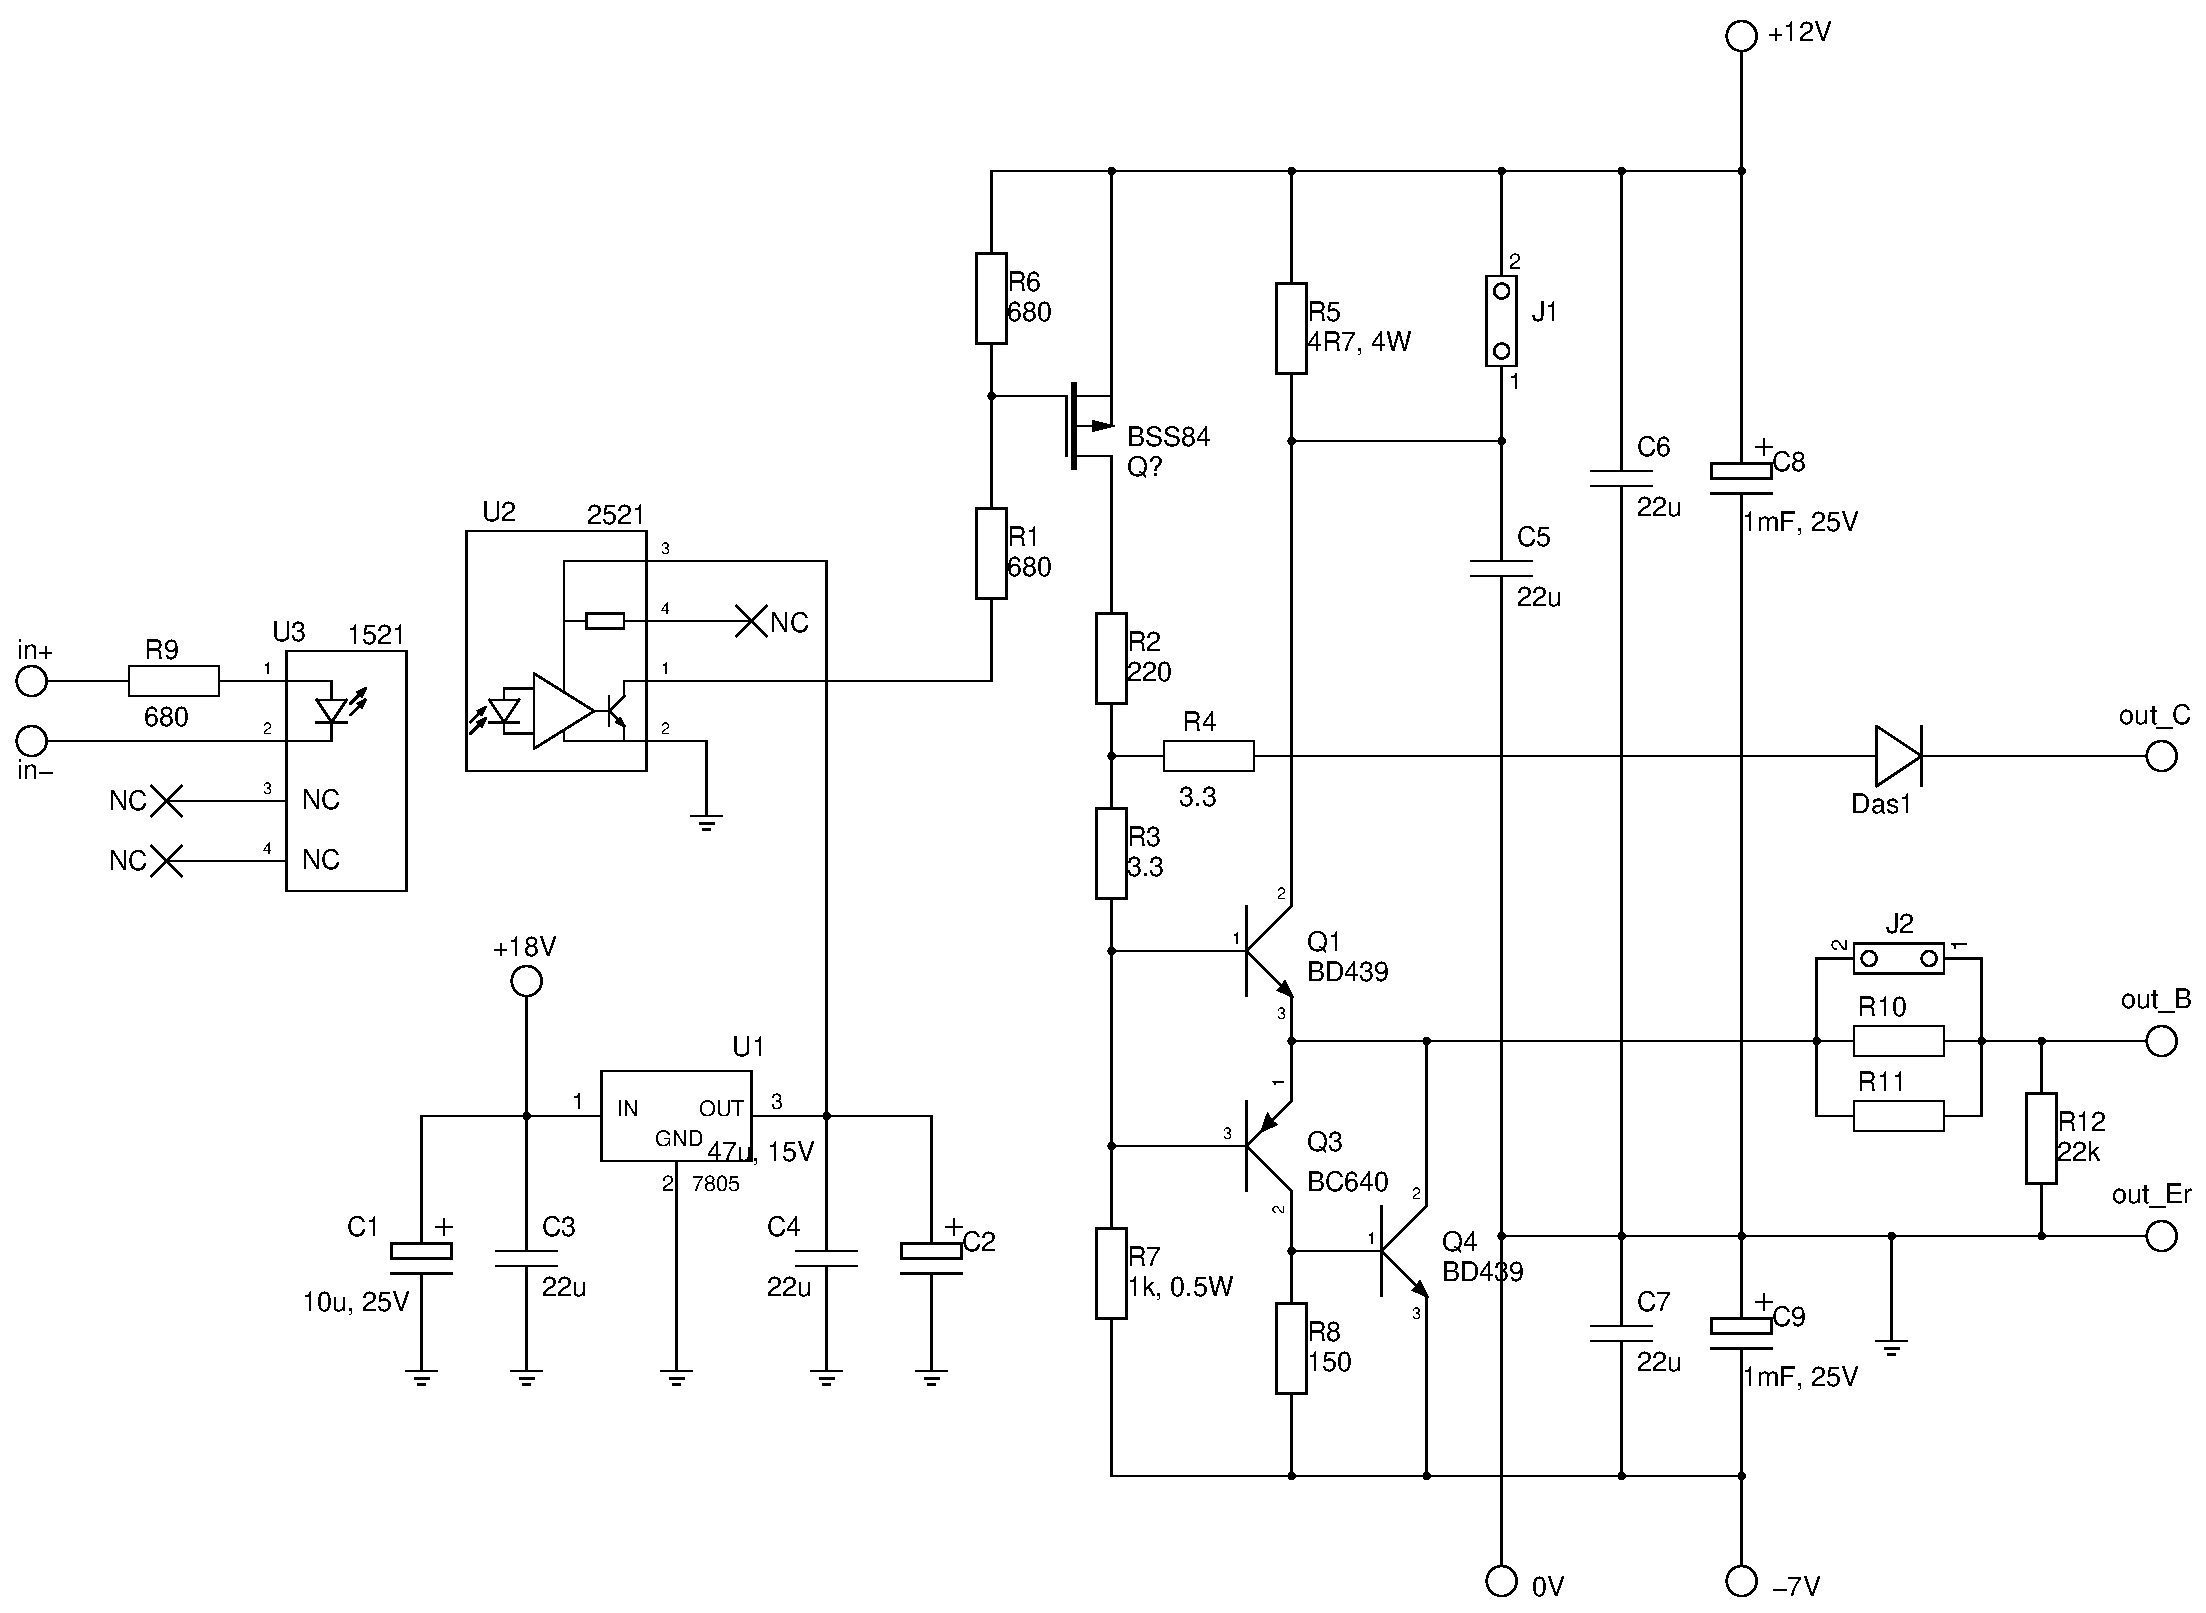
\includegraphics[height=.8\textheight]{../obr/schema_budic2}

\section{Obvodová schéma budiča generátora impulzov}
\hspace{-1.8cm}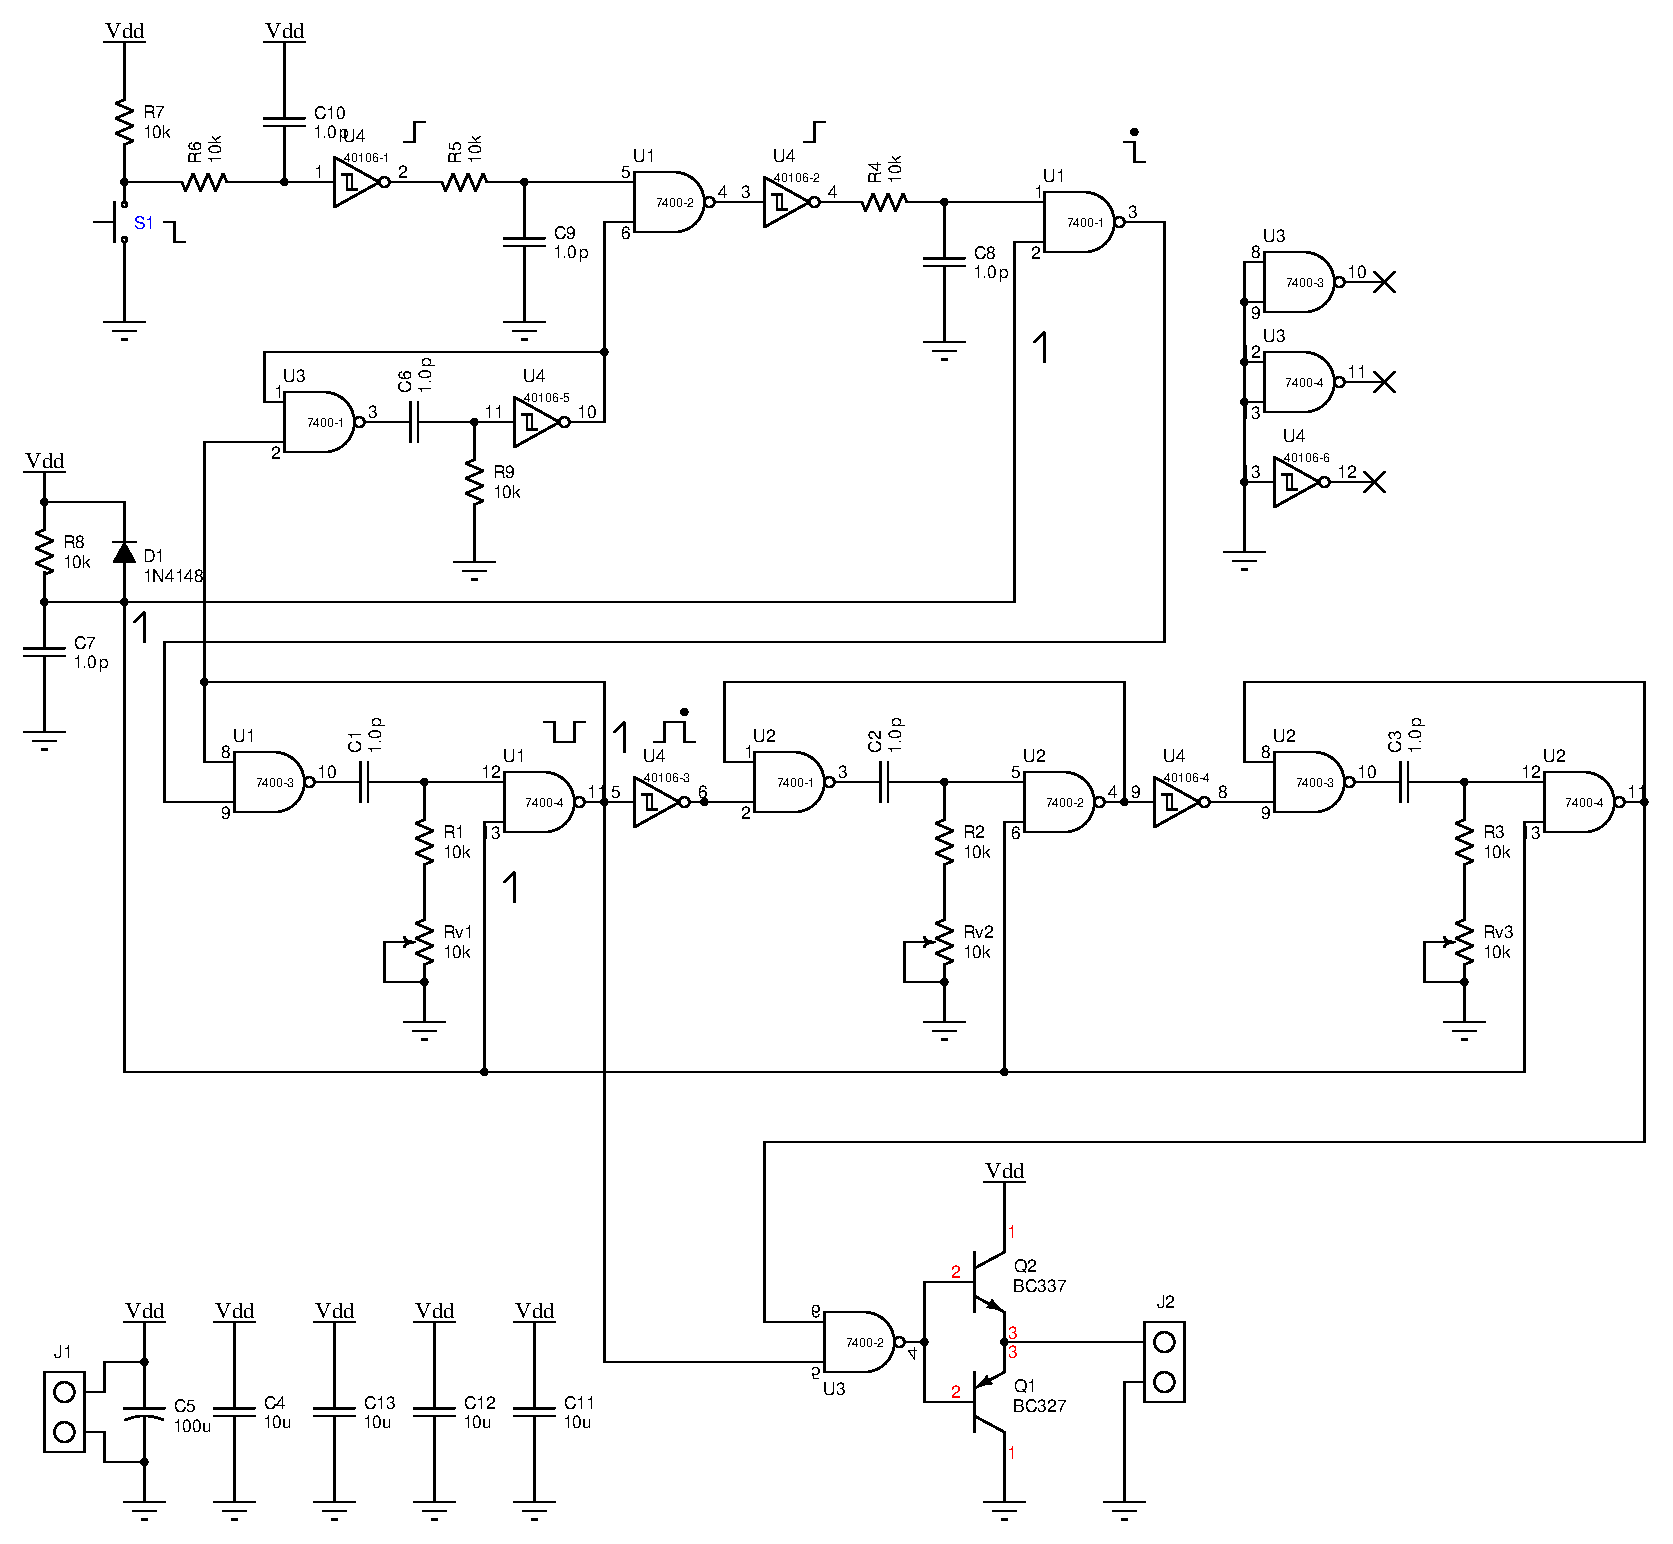
\includegraphics[height=.8\textheight]{../obr/schema_gen}


\label{LastPage}
\end{document}
